\documentclass[1p]{elsarticle_modified}
%\bibliographystyle{elsarticle-num}

%\usepackage[colorlinks]{hyperref}
%\usepackage{abbrmath_seonhwa} %\Abb, \Ascr, \Acal ,\Abf, \Afrak
\usepackage{amsfonts}
\usepackage{amssymb}
\usepackage{amsmath}
\usepackage{amsthm}
\usepackage{scalefnt}
\usepackage{amsbsy}
\usepackage{kotex}
\usepackage{caption}
\usepackage{subfig}
\usepackage{color}
\usepackage{graphicx}
\usepackage{xcolor} %% white, black, red, green, blue, cyan, magenta, yellow
\usepackage{float}
\usepackage{setspace}
\usepackage{hyperref}

\usepackage{tikz}
\usetikzlibrary{arrows}

\usepackage{multirow}
\usepackage{array} % fixed length table
\usepackage{hhline}

%%%%%%%%%%%%%%%%%%%%%
\makeatletter
\renewcommand*\env@matrix[1][\arraystretch]{%
	\edef\arraystretch{#1}%
	\hskip -\arraycolsep
	\let\@ifnextchar\new@ifnextchar
	\array{*\c@MaxMatrixCols c}}
\makeatother %https://tex.stackexchange.com/questions/14071/how-can-i-increase-the-line-spacing-in-a-matrix
%%%%%%%%%%%%%%%

\usepackage[normalem]{ulem}

\newcommand{\msout}[1]{\ifmmode\text{\sout{\ensuremath{#1}}}\else\sout{#1}\fi}
%SOURCE: \msout is \stkout macro in https://tex.stackexchange.com/questions/20609/strikeout-in-math-mode

\newcommand{\cancel}[1]{
	\ifmmode
	{\color{red}\msout{#1}}
	\else
	{\color{red}\sout{#1}}
	\fi
}

\newcommand{\add}[1]{
	{\color{blue}\uwave{#1}}
}

\newcommand{\replace}[2]{
	\ifmmode
	{\color{red}\msout{#1}}{\color{blue}\uwave{#2}}
	\else
	{\color{red}\sout{#1}}{\color{blue}\uwave{#2}}
	\fi
}

\newcommand{\Sol}{\mathcal{S}} %segment
\newcommand{\D}{D} %diagram
\newcommand{\A}{\mathcal{A}} %arc


%%%%%%%%%%%%%%%%%%%%%%%%%%%%%5 test

\def\sl{\operatorname{\textup{SL}}(2,\Cbb)}
\def\psl{\operatorname{\textup{PSL}}(2,\Cbb)}
\def\quan{\mkern 1mu \triangleright \mkern 1mu}

\theoremstyle{definition}
\newtheorem{thm}{Theorem}[section]
\newtheorem{prop}[thm]{Proposition}
\newtheorem{lem}[thm]{Lemma}
\newtheorem{ques}[thm]{Question}
\newtheorem{cor}[thm]{Corollary}
\newtheorem{defn}[thm]{Definition}
\newtheorem{exam}[thm]{Example}
\newtheorem{rmk}[thm]{Remark}
\newtheorem{alg}[thm]{Algorithm}

\newcommand{\I}{\sqrt{-1}}
\begin{document}

%\begin{frontmatter}
%
%\title{Boundary parabolic representations of knots up to 8 crossings}
%
%%% Group authors per affiliation:
%\author{Yunhi Cho} 
%\address{Department of Mathematics, University of Seoul, Seoul, Korea}
%\ead{yhcho@uos.ac.kr}
%
%
%\author{Seonhwa Kim} %\fnref{s_kim}}
%\address{Center for Geometry and Physics, Institute for Basic Science, Pohang, 37673, Korea}
%\ead{ryeona17@ibs.re.kr}
%
%\author{Hyuk Kim}
%\address{Department of Mathematical Sciences, Seoul National University, Seoul 08826, Korea}
%\ead{hyukkim@snu.ac.kr}
%
%\author{Seokbeom Yoon}
%\address{Department of Mathematical Sciences, Seoul National University, Seoul, 08826,  Korea}
%\ead{sbyoon15@snu.ac.kr}
%
%\begin{abstract}
%We find all boundary parabolic representation of knots up to 8 crossings.
%
%\end{abstract}
%\begin{keyword}
%    \MSC[2010] 57M25 
%\end{keyword}
%
%\end{frontmatter}

%\linenumbers
%\tableofcontents
%
\newcommand\colored[1]{\textcolor{white}{\rule[-0.35ex]{0.8em}{1.4ex}}\kern-0.8em\color{red} #1}%
%\newcommand\colored[1]{\textcolor{white}{ #1}\kern-2.17ex	\textcolor{white}{ #1}\kern-1.81ex	\textcolor{white}{ #1}\kern-2.15ex\color{red}#1	}

{\Large $\underline{12n_{0541}~(K12n_{0541})}$}

\setlength{\tabcolsep}{10pt}
\renewcommand{\arraystretch}{1.6}
\vspace{1cm}\begin{tabular}{m{100pt}>{\centering\arraybackslash}m{274pt}}
\multirow{5}{120pt}{
	\centering
	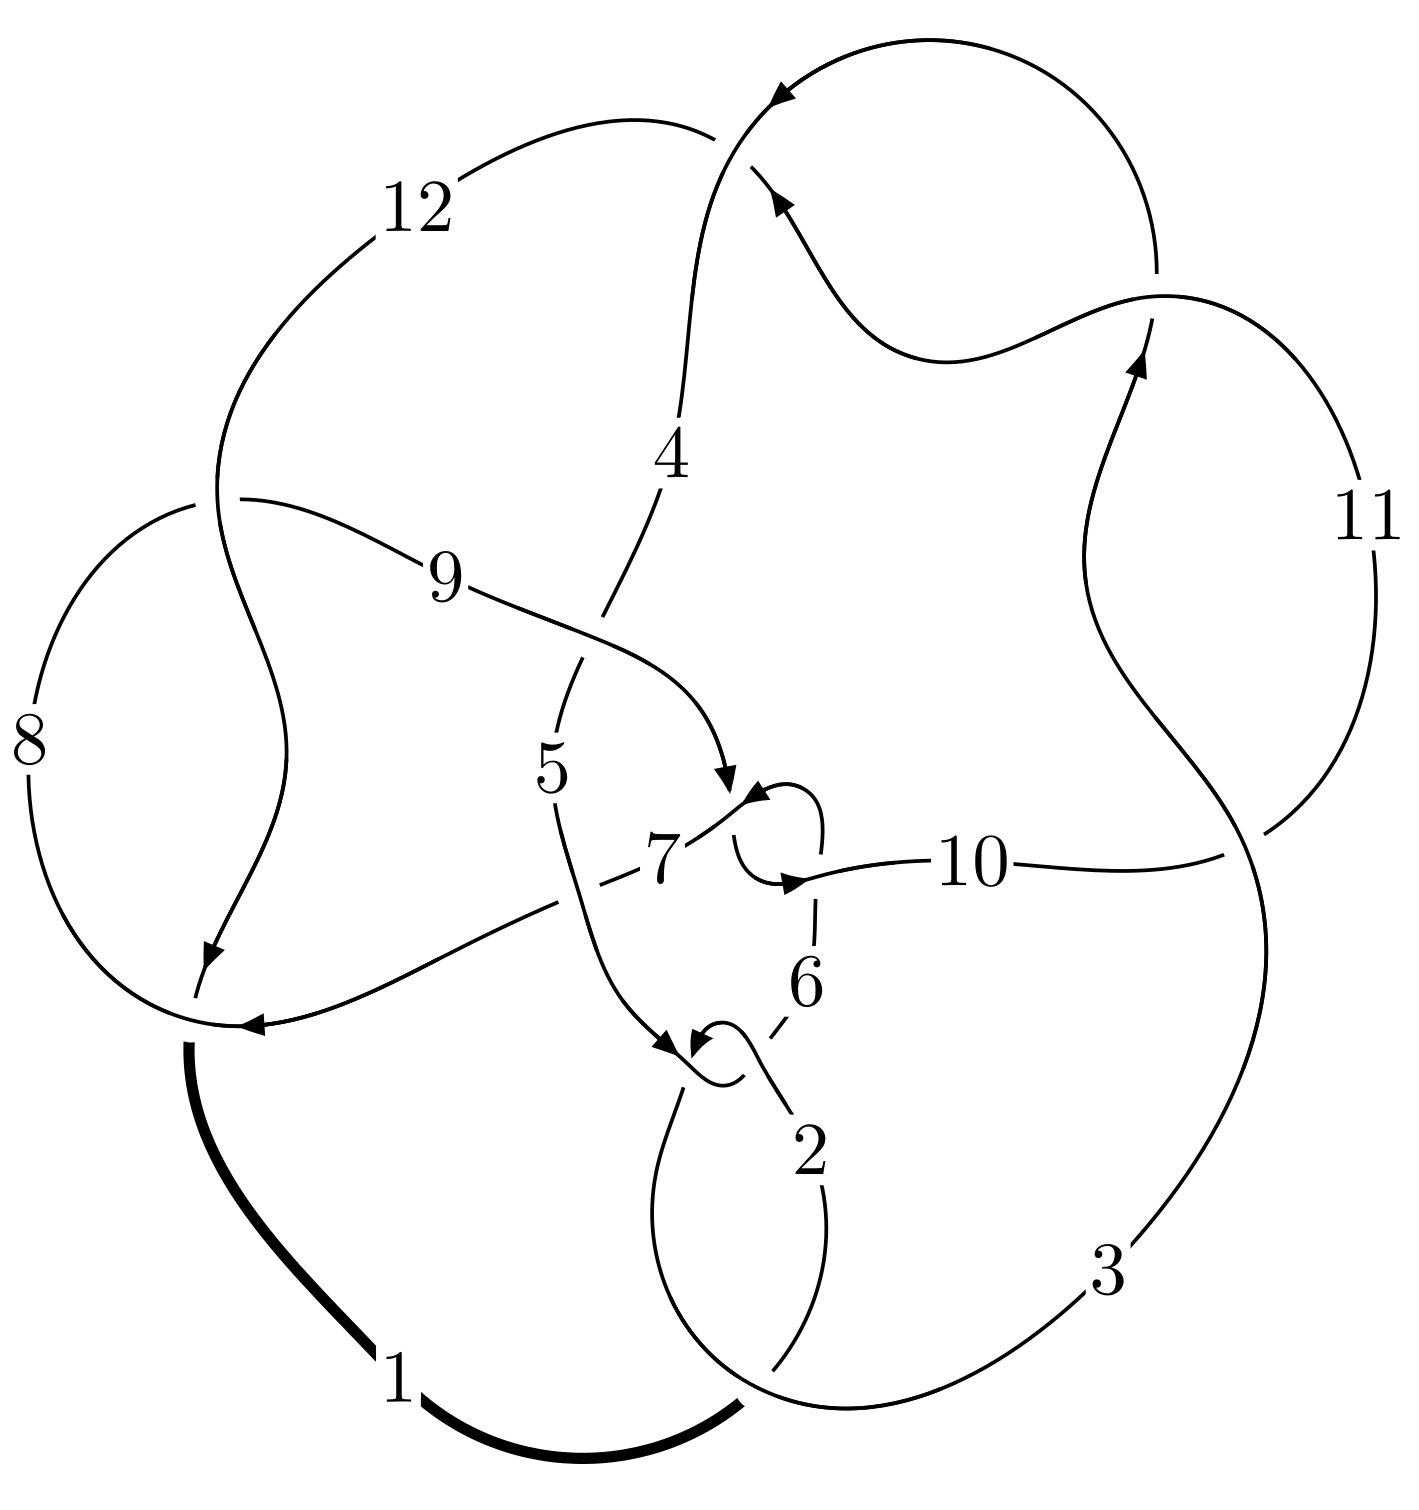
\includegraphics[width=112pt]{../../../GIT/diagram.site/Diagrams/png/2630_12n_0541.png}\\
\ \ \ A knot diagram\footnotemark}&
\allowdisplaybreaks
\textbf{Linearized knot diagam} \\
\cline{2-2}
 &
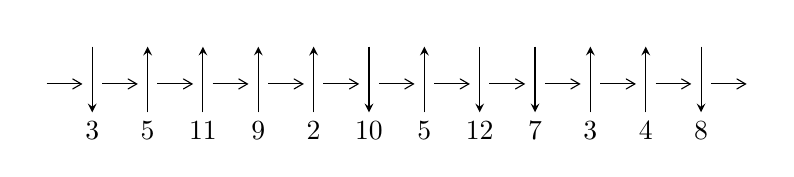
\begin{tikzpicture}[x=20pt, y=17pt]
	% nodes
	\node (C0) at (0, 0) {};
	\node (C1) at (1, 0) {};
	\node (C1U) at (1, +1) {};
	\node (C1D) at (1, -1) {3};

	\node (C2) at (2, 0) {};
	\node (C2U) at (2, +1) {};
	\node (C2D) at (2, -1) {5};

	\node (C3) at (3, 0) {};
	\node (C3U) at (3, +1) {};
	\node (C3D) at (3, -1) {11};

	\node (C4) at (4, 0) {};
	\node (C4U) at (4, +1) {};
	\node (C4D) at (4, -1) {9};

	\node (C5) at (5, 0) {};
	\node (C5U) at (5, +1) {};
	\node (C5D) at (5, -1) {2};

	\node (C6) at (6, 0) {};
	\node (C6U) at (6, +1) {};
	\node (C6D) at (6, -1) {10};

	\node (C7) at (7, 0) {};
	\node (C7U) at (7, +1) {};
	\node (C7D) at (7, -1) {5};

	\node (C8) at (8, 0) {};
	\node (C8U) at (8, +1) {};
	\node (C8D) at (8, -1) {12};

	\node (C9) at (9, 0) {};
	\node (C9U) at (9, +1) {};
	\node (C9D) at (9, -1) {7};

	\node (C10) at (10, 0) {};
	\node (C10U) at (10, +1) {};
	\node (C10D) at (10, -1) {3};

	\node (C11) at (11, 0) {};
	\node (C11U) at (11, +1) {};
	\node (C11D) at (11, -1) {4};

	\node (C12) at (12, 0) {};
	\node (C12U) at (12, +1) {};
	\node (C12D) at (12, -1) {8};
	\node (C13) at (13, 0) {};

	% arrows
	\draw[->,>={angle 60}]
	(C0) edge (C1) (C1) edge (C2) (C2) edge (C3) (C3) edge (C4) (C4) edge (C5) (C5) edge (C6) (C6) edge (C7) (C7) edge (C8) (C8) edge (C9) (C9) edge (C10) (C10) edge (C11) (C11) edge (C12) (C12) edge (C13) ;	\draw[->,>=stealth]
	(C1U) edge (C1D) (C2D) edge (C2U) (C3D) edge (C3U) (C4D) edge (C4U) (C5D) edge (C5U) (C6U) edge (C6D) (C7D) edge (C7U) (C8U) edge (C8D) (C9U) edge (C9D) (C10D) edge (C10U) (C11D) edge (C11U) (C12U) edge (C12D) ;
	\end{tikzpicture} \\
\hhline{~~} \\& 
\textbf{Solving Sequence} \\ \cline{2-2} 
 &
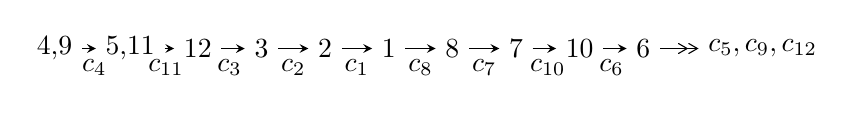
\begin{tikzpicture}[x=23pt, y=7pt]
	% node
	\node (A0) at (-1/8, 0) {4,9};
	\node (A1) at (17/16, 0) {5,11};
	\node (A2) at (17/8, 0) {12};
	\node (A3) at (25/8, 0) {3};
	\node (A4) at (33/8, 0) {2};
	\node (A5) at (41/8, 0) {1};
	\node (A6) at (49/8, 0) {8};
	\node (A7) at (57/8, 0) {7};
	\node (A8) at (65/8, 0) {10};
	\node (A9) at (73/8, 0) {6};
	\node (C1) at (1/2, -1) {$c_{4}$};
	\node (C2) at (13/8, -1) {$c_{11}$};
	\node (C3) at (21/8, -1) {$c_{3}$};
	\node (C4) at (29/8, -1) {$c_{2}$};
	\node (C5) at (37/8, -1) {$c_{1}$};
	\node (C6) at (45/8, -1) {$c_{8}$};
	\node (C7) at (53/8, -1) {$c_{7}$};
	\node (C8) at (61/8, -1) {$c_{10}$};
	\node (C9) at (69/8, -1) {$c_{6}$};
	\node (A10) at (11, 0) {$c_{5},c_{9},c_{12}$};

	% edge
	\draw[->,>=stealth]	
	(A0) edge (A1) (A1) edge (A2) (A2) edge (A3) (A3) edge (A4) (A4) edge (A5) (A5) edge (A6) (A6) edge (A7) (A7) edge (A8) (A8) edge (A9) ;
	\draw[->>,>={angle 60}]	
	(A9) edge (A10);
\end{tikzpicture} \\ 

\end{tabular} \\

\footnotetext{
The image of knot diagram is generated by the software ``\textbf{Draw programme}" developed by Andrew Bartholomew(\url{http://www.layer8.co.uk/maths/draw/index.htm\#Running-draw}), where we modified some parts for our purpose(\url{https://github.com/CATsTAILs/LinksPainter}).
}\phantom \\ \newline 
\centering \textbf{Ideals for irreducible components\footnotemark of $X_{\text{par}}$} 
 
\begin{align*}
I^u_{1}&=\langle 
-5.87639\times10^{132} u^{57}+2.50106\times10^{132} u^{56}+\cdots+2.99453\times10^{133} b-8.33073\times10^{134},\\
\phantom{I^u_{1}}&\phantom{= \langle  }2.36705\times10^{135} u^{57}-2.44899\times10^{134} u^{56}+\cdots+2.90469\times10^{135} a+2.58804\times10^{137},\\
\phantom{I^u_{1}}&\phantom{= \langle  }u^{58}- u^{57}+\cdots+1784 u-97\rangle \\
I^u_{2}&=\langle 
8348 u^{16}+3209 u^{15}+\cdots+199783 b+57302,\;-39879 u^{16}+47300 u^{15}+\cdots+199783 a+155745,\\
\phantom{I^u_{2}}&\phantom{= \langle  }u^{17}-2 u^{16}+\cdots- u+1\rangle \\
\\
\end{align*}
\raggedright * 2 irreducible components of $\dim_{\mathbb{C}}=0$, with total 75 representations.\\
\footnotetext{All coefficients of polynomials are rational numbers. But the coefficients are sometimes approximated in decimal forms when there is not enough margin.}
\newpage
\renewcommand{\arraystretch}{1}
\centering \section*{I. $I^u_{1}= \langle -5.88\times10^{132} u^{57}+2.50\times10^{132} u^{56}+\cdots+2.99\times10^{133} b-8.33\times10^{134},\;2.37\times10^{135} u^{57}-2.45\times10^{134} u^{56}+\cdots+2.90\times10^{135} a+2.59\times10^{137},\;u^{58}- u^{57}+\cdots+1784 u-97 \rangle$}
\flushleft \textbf{(i) Arc colorings}\\
\begin{tabular}{m{7pt} m{180pt} m{7pt} m{180pt} }
\flushright $a_{4}=$&$\begin{pmatrix}1\\0\end{pmatrix}$ \\
\flushright $a_{9}=$&$\begin{pmatrix}0\\u\end{pmatrix}$ \\
\flushright $a_{5}=$&$\begin{pmatrix}1\\- u^2\end{pmatrix}$ \\
\flushright $a_{11}=$&$\begin{pmatrix}-0.814905 u^{57}+0.0843114 u^{56}+\cdots+1564.87 u-89.0986\\0.196237 u^{57}-0.0835210 u^{56}+\cdots-465.329 u+27.8198\end{pmatrix}$ \\
\flushright $a_{12}=$&$\begin{pmatrix}-0.618667 u^{57}+0.000790408 u^{56}+\cdots+1099.54 u-61.2788\\0.196237 u^{57}-0.0835210 u^{56}+\cdots-465.329 u+27.8198\end{pmatrix}$ \\
\flushright $a_{3}=$&$\begin{pmatrix}1.26264 u^{57}-0.178664 u^{56}+\cdots-2319.14 u+134.740\\-0.886420 u^{57}+0.185562 u^{56}+\cdots+1779.38 u-102.951\end{pmatrix}$ \\
\flushright $a_{2}=$&$\begin{pmatrix}1.24998 u^{57}-0.173335 u^{56}+\cdots-2287.18 u+132.545\\-0.876439 u^{57}+0.192317 u^{56}+\cdots+1767.53 u-102.241\end{pmatrix}$ \\
\flushright $a_{1}=$&$\begin{pmatrix}-1.47512 u^{57}+0.219193 u^{56}+\cdots+3001.64 u-177.485\\1.07633 u^{57}-0.215056 u^{56}+\cdots-2148.64 u+124.617\end{pmatrix}$ \\
\flushright $a_{8}=$&$\begin{pmatrix}-1.24859 u^{57}+0.152603 u^{56}+\cdots+2443.79 u-145.739\\0.383117 u^{57}-0.00368130 u^{56}+\cdots-639.387 u+36.4933\end{pmatrix}$ \\
\flushright $a_{7}=$&$\begin{pmatrix}-0.680762 u^{57}+0.0174945 u^{56}+\cdots+1249.05 u-75.9216\\0.0844112 u^{57}+0.117389 u^{56}+\cdots+77.5028 u-5.48038\end{pmatrix}$ \\
\flushright $a_{10}=$&$\begin{pmatrix}1.24700 u^{57}-0.233097 u^{56}+\cdots-2487.40 u+146.530\\-1.82228 u^{57}+0.192500 u^{56}+\cdots+3348.40 u-192.831\end{pmatrix}$ \\
\flushright $a_{6}=$&$\begin{pmatrix}1.14160 u^{57}+0.209026 u^{56}+\cdots-1445.32 u+77.9733\\-1.50016 u^{57}-0.128282 u^{56}+\cdots+2270.12 u-129.468\end{pmatrix}$\\&\end{tabular}
\flushleft \textbf{(ii) Obstruction class $= -1$}\\~\\
\flushleft \textbf{(iii) Cusp Shapes $= -0.0616248 u^{57}+0.0782720 u^{56}+\cdots+282.553 u-10.0154$}\\~\\
\newpage\renewcommand{\arraystretch}{1}
\flushleft \textbf{(iv) u-Polynomials at the component}\newline \\
\begin{tabular}{m{50pt}|m{274pt}}
Crossings & \hspace{64pt}u-Polynomials at each crossing \\
\hline $$\begin{aligned}c_{1}\end{aligned}$$&$\begin{aligned}
&u^{58}+57 u^{57}+\cdots-77375 u+361
\end{aligned}$\\
\hline $$\begin{aligned}c_{2},c_{5}\end{aligned}$$&$\begin{aligned}
&u^{58}+3 u^{57}+\cdots+293 u-19
\end{aligned}$\\
\hline $$\begin{aligned}c_{3},c_{10},c_{11}\end{aligned}$$&$\begin{aligned}
&u^{58}-2 u^{57}+\cdots-334 u+116
\end{aligned}$\\
\hline $$\begin{aligned}c_{4}\end{aligned}$$&$\begin{aligned}
&u^{58}- u^{57}+\cdots+1784 u-97
\end{aligned}$\\
\hline $$\begin{aligned}c_{6},c_{9}\end{aligned}$$&$\begin{aligned}
&u^{58}-4 u^{57}+\cdots-11 u+1
\end{aligned}$\\
\hline $$\begin{aligned}c_{7}\end{aligned}$$&$\begin{aligned}
&u^{58}+7 u^{57}+\cdots-31992 u-20788
\end{aligned}$\\
\hline $$\begin{aligned}c_{8},c_{12}\end{aligned}$$&$\begin{aligned}
&u^{58}+u^{57}+\cdots+14968 u-1819
\end{aligned}$\\
\hline
\end{tabular}\\~\\
\newpage\renewcommand{\arraystretch}{1}
\flushleft \textbf{(v) Riley Polynomials at the component}\newline \\
\begin{tabular}{m{50pt}|m{274pt}}
Crossings & \hspace{64pt}Riley Polynomials at each crossing \\
\hline $$\begin{aligned}c_{1}\end{aligned}$$&$\begin{aligned}
&y^{58}-151 y^{57}+\cdots-8652137019 y+130321
\end{aligned}$\\
\hline $$\begin{aligned}c_{2},c_{5}\end{aligned}$$&$\begin{aligned}
&y^{58}+57 y^{57}+\cdots-77375 y+361
\end{aligned}$\\
\hline $$\begin{aligned}c_{3},c_{10},c_{11}\end{aligned}$$&$\begin{aligned}
&y^{58}-54 y^{57}+\cdots+91908 y+13456
\end{aligned}$\\
\hline $$\begin{aligned}c_{4}\end{aligned}$$&$\begin{aligned}
&y^{58}-35 y^{57}+\cdots-1420360 y+9409
\end{aligned}$\\
\hline $$\begin{aligned}c_{6},c_{9}\end{aligned}$$&$\begin{aligned}
&y^{58}+18 y^{57}+\cdots-5 y+1
\end{aligned}$\\
\hline $$\begin{aligned}c_{7}\end{aligned}$$&$\begin{aligned}
&y^{58}-23 y^{57}+\cdots-4796634792 y+432140944
\end{aligned}$\\
\hline $$\begin{aligned}c_{8},c_{12}\end{aligned}$$&$\begin{aligned}
&y^{58}+33 y^{57}+\cdots+9212984 y+3308761
\end{aligned}$\\
\hline
\end{tabular}\\~\\
\newpage\flushleft \textbf{(vi) Complex Volumes and Cusp Shapes}
$$\begin{array}{c|c|c}  
\text{Solutions to }I^u_{1}& \I (\text{vol} + \sqrt{-1}CS) & \text{Cusp shape}\\
 \hline 
\begin{aligned}
u &= \phantom{-}0.940914 + 0.335118 I \\
a &= \phantom{-}0.070878 + 0.648829 I \\
b &= \phantom{-}0.333376 + 0.570263 I\end{aligned}
 & \phantom{-}1.77937 + 1.64554 I & \phantom{-}2.35543 - 4.26345 I \\ \hline\begin{aligned}
u &= \phantom{-}0.940914 - 0.335118 I \\
a &= \phantom{-}0.070878 - 0.648829 I \\
b &= \phantom{-}0.333376 - 0.570263 I\end{aligned}
 & \phantom{-}1.77937 - 1.64554 I & \phantom{-}2.35543 + 4.26345 I \\ \hline\begin{aligned}
u &= \phantom{-}0.533417 + 0.837553 I \\
a &= -1.203420 - 0.385244 I \\
b &= \phantom{-}0.000815 + 0.660806 I\end{aligned}
 & -6.45413 - 3.97977 I & -0.21992 + 1.71785 I \\ \hline\begin{aligned}
u &= \phantom{-}0.533417 - 0.837553 I \\
a &= -1.203420 + 0.385244 I \\
b &= \phantom{-}0.000815 - 0.660806 I\end{aligned}
 & -6.45413 + 3.97977 I & -0.21992 - 1.71785 I \\ \hline\begin{aligned}
u &= \phantom{-}0.965855 + 0.129569 I \\
a &= \phantom{-}1.113392 + 0.042885 I \\
b &= -1.21907 + 0.95214 I\end{aligned}
 & -2.00228 + 1.64608 I & \phantom{-}6.20898 - 1.56936 I \\ \hline\begin{aligned}
u &= \phantom{-}0.965855 - 0.129569 I \\
a &= \phantom{-}1.113392 - 0.042885 I \\
b &= -1.21907 - 0.95214 I\end{aligned}
 & -2.00228 - 1.64608 I & \phantom{-}6.20898 + 1.56936 I \\ \hline\begin{aligned}
u &= -1.007521 + 0.242272 I \\
a &= -0.829841 + 0.512646 I \\
b &= \phantom{-}0.530354 + 0.625433 I\end{aligned}
 & \phantom{-}4.33258 - 1.31394 I & \phantom{-}8.82093 - 0.72054 I \\ \hline\begin{aligned}
u &= -1.007521 - 0.242272 I \\
a &= -0.829841 - 0.512646 I \\
b &= \phantom{-}0.530354 - 0.625433 I\end{aligned}
 & \phantom{-}4.33258 + 1.31394 I & \phantom{-}8.82093 + 0.72054 I \\ \hline\begin{aligned}
u &= \phantom{-}0.651210 + 0.709503 I \\
a &= \phantom{-}0.763151 - 0.282177 I \\
b &= -0.553097 - 0.053434 I\end{aligned}
 & \phantom{-}0.84503 + 2.28235 I & -1.95290 - 6.63736 I \\ \hline\begin{aligned}
u &= \phantom{-}0.651210 - 0.709503 I \\
a &= \phantom{-}0.763151 + 0.282177 I \\
b &= -0.553097 + 0.053434 I\end{aligned}
 & \phantom{-}0.84503 - 2.28235 I & -1.95290 + 6.63736 I\\
 \hline 
 \end{array}$$\newpage$$\begin{array}{c|c|c}  
\text{Solutions to }I^u_{1}& \I (\text{vol} + \sqrt{-1}CS) & \text{Cusp shape}\\
 \hline 
\begin{aligned}
u &= \phantom{-}0.925221 + 0.121993 I \\
a &= \phantom{-}2.81123 + 0.85530 I \\
b &= -1.335825 - 0.306901 I\end{aligned}
 & -2.16189 - 0.49659 I & \phantom{-}5.68631 - 0.44795 I \\ \hline\begin{aligned}
u &= \phantom{-}0.925221 - 0.121993 I \\
a &= \phantom{-}2.81123 - 0.85530 I \\
b &= -1.335825 + 0.306901 I\end{aligned}
 & -2.16189 + 0.49659 I & \phantom{-}5.68631 + 0.44795 I \\ \hline\begin{aligned}
u &= -0.871211 + 0.645662 I \\
a &= \phantom{-}                -6
0.488418 + 6. 10   I \\
b &= -0.408786 + 1.020246 I\end{aligned}
 & -6.33690 - 1.89605 I & \phantom{-0.000000 -}0. + 3.04775 I \\ \hline\begin{aligned}
u &= -0.871211 - 0.645662 I \\
a &= \phantom{-}                -6
0.488418 - 6. 10   I \\
b &= -0.408786 - 1.020246 I\end{aligned}
 & -6.33690 + 1.89605 I & \phantom{-0.000000 } 0. - 3.04775 I \\ \hline\begin{aligned}
u &= -1.050300 + 0.294172 I \\
a &= \phantom{-}2.71489 - 0.03928 I \\
b &= -1.272275 + 0.309727 I\end{aligned}
 & -3.03611 - 7.19983 I & \phantom{-}4.74744 + 5.63439 I \\ \hline\begin{aligned}
u &= -1.050300 - 0.294172 I \\
a &= \phantom{-}2.71489 + 0.03928 I \\
b &= -1.272275 - 0.309727 I\end{aligned}
 & -3.03611 + 7.19983 I & \phantom{-}4.74744 - 5.63439 I \\ \hline\begin{aligned}
u &= -1.010203 + 0.412736 I \\
a &= \phantom{-}1.52613 + 1.10002 I \\
b &= -1.65214 + 0.15953 I\end{aligned}
 & \phantom{-}12.04110 - 1.74691 I & \phantom{-}11.96174 + 0. I\phantom{ +0.000000I} \\ \hline\begin{aligned}
u &= -1.010203 - 0.412736 I \\
a &= \phantom{-}1.52613 - 1.10002 I \\
b &= -1.65214 - 0.15953 I\end{aligned}
 & \phantom{-}12.04110 + 1.74691 I & \phantom{-}11.96174 + 0. I\phantom{ +0.000000I} \\ \hline\begin{aligned}
u &= \phantom{-}1.070601 + 0.256261 I \\
a &= \phantom{-}0.212194 + 0.279123 I \\
b &= \phantom{-}0.232507 + 0.484962 I\end{aligned}
 & \phantom{-}1.89676 + 1.25482 I & \phantom{-}2.00000 + 0. I\phantom{ +0.000000I} \\ \hline\begin{aligned}
u &= \phantom{-}1.070601 - 0.256261 I \\
a &= \phantom{-}0.212194 - 0.279123 I \\
b &= \phantom{-}0.232507 - 0.484962 I\end{aligned}
 & \phantom{-}1.89676 - 1.25482 I & \phantom{-}2.00000 + 0. I\phantom{ +0.000000I}\\
 \hline 
 \end{array}$$\newpage$$\begin{array}{c|c|c}  
\text{Solutions to }I^u_{1}& \I (\text{vol} + \sqrt{-1}CS) & \text{Cusp shape}\\
 \hline 
\begin{aligned}
u &= -0.764087 + 0.799193 I \\
a &= -0.835657 + 0.390939 I \\
b &= -0.074847 - 0.721706 I\end{aligned}
 & -6.80237 - 3.50038 I & \phantom{-0.000000 -}0. + 2.31257 I \\ \hline\begin{aligned}
u &= -0.764087 - 0.799193 I \\
a &= -0.835657 - 0.390939 I \\
b &= -0.074847 + 0.721706 I\end{aligned}
 & -6.80237 + 3.50038 I & \phantom{-0.000000 } 0. - 2.31257 I \\ \hline\begin{aligned}
u &= \phantom{-}1.080654 + 0.302294 I \\
a &= -1.10389 + 1.63263 I \\
b &= \phantom{-}1.110899 + 0.164797 I\end{aligned}
 & \phantom{-}3.68955 + 0.99282 I & \phantom{-0.000000 -}0. + 5.78441 I \\ \hline\begin{aligned}
u &= \phantom{-}1.080654 - 0.302294 I \\
a &= -1.10389 - 1.63263 I \\
b &= \phantom{-}1.110899 - 0.164797 I\end{aligned}
 & \phantom{-}3.68955 - 0.99282 I & \phantom{-0.000000 } 0. - 5.78441 I \\ \hline\begin{aligned}
u &= \phantom{-}1.12582\phantom{ +0.000000I} \\
a &= -3.41567\phantom{ +0.000000I} \\
b &= \phantom{-}1.14657\phantom{ +0.000000I}\end{aligned}
 & \phantom{-}3.83802\phantom{ +0.000000I} & -56.3460\phantom{ +0.000000I} \\ \hline\begin{aligned}
u &= -0.855805\phantom{ +0.000000I} \\
a &= -2.49525\phantom{ +0.000000I} \\
b &= \phantom{-}1.31986\phantom{ +0.000000I}\end{aligned}
 & \phantom{-}2.77980\phantom{ +0.000000I} & -0.400550\phantom{ +0.000000I} \\ \hline\begin{aligned}
u &= \phantom{-}1.034985 + 0.489339 I \\
a &= -1.84386 + 0.74811 I \\
b &= \phantom{-}1.76254 + 0.04368 I\end{aligned}
 & \phantom{-}9.76113 + 2.08154 I & \phantom{-0.000000 } 0 \\ \hline\begin{aligned}
u &= \phantom{-}1.034985 - 0.489339 I \\
a &= -1.84386 - 0.74811 I \\
b &= \phantom{-}1.76254 - 0.04368 I\end{aligned}
 & \phantom{-}9.76113 - 2.08154 I & \phantom{-0.000000 } 0 \\ \hline\begin{aligned}
u &= \phantom{-}1.125366 + 0.516938 I \\
a &= \phantom{-}0.355709 + 0.158453 I \\
b &= -0.341555 - 1.213756 I\end{aligned}
 & -4.45556 + 9.01614 I & \phantom{-0.000000 } 0 \\ \hline\begin{aligned}
u &= \phantom{-}1.125366 - 0.516938 I \\
a &= \phantom{-}0.355709 - 0.158453 I \\
b &= -0.341555 + 1.213756 I\end{aligned}
 & -4.45556 - 9.01614 I & \phantom{-0.000000 } 0\\
 \hline 
 \end{array}$$\newpage$$\begin{array}{c|c|c}  
\text{Solutions to }I^u_{1}& \I (\text{vol} + \sqrt{-1}CS) & \text{Cusp shape}\\
 \hline 
\begin{aligned}
u &= -0.583369 + 0.471942 I \\
a &= \phantom{-}0.906827 - 0.159977 I \\
b &= -1.056792 - 0.724510 I\end{aligned}
 & -4.47025 + 4.18059 I & \phantom{-}3.66036 + 0.35432 I \\ \hline\begin{aligned}
u &= -0.583369 - 0.471942 I \\
a &= \phantom{-}0.906827 + 0.159977 I \\
b &= -1.056792 + 0.724510 I\end{aligned}
 & -4.47025 - 4.18059 I & \phantom{-}3.66036 - 0.35432 I \\ \hline\begin{aligned}
u &= -0.642745 + 1.117227 I \\
a &= -0.677478 - 0.528065 I \\
b &= \phantom{-}1.38029 + 0.34754 I\end{aligned}
 & -2.13403 + 0.38137 I & \phantom{-0.000000 } 0 \\ \hline\begin{aligned}
u &= -0.642745 - 1.117227 I \\
a &= -0.677478 + 0.528065 I \\
b &= \phantom{-}1.38029 - 0.34754 I\end{aligned}
 & -2.13403 - 0.38137 I & \phantom{-0.000000 } 0 \\ \hline\begin{aligned}
u &= -1.266436 + 0.283598 I \\
a &= -0.231931 - 0.055908 I \\
b &= \phantom{-}0.115661 - 0.792769 I\end{aligned}
 & \phantom{-}2.77371 - 4.65817 I & \phantom{-0.000000 } 0 \\ \hline\begin{aligned}
u &= -1.266436 - 0.283598 I \\
a &= -0.231931 + 0.055908 I \\
b &= \phantom{-}0.115661 + 0.792769 I\end{aligned}
 & \phantom{-}2.77371 + 4.65817 I & \phantom{-0.000000 } 0 \\ \hline\begin{aligned}
u &= \phantom{-}0.133420 + 1.293482 I \\
a &= \phantom{-}0.506063 - 0.156731 I \\
b &= -1.212023 - 0.070395 I\end{aligned}
 & \phantom{-}2.31699 + 2.80503 I & \phantom{-0.000000 } 0 \\ \hline\begin{aligned}
u &= \phantom{-}0.133420 - 1.293482 I \\
a &= \phantom{-}0.506063 + 0.156731 I \\
b &= -1.212023 + 0.070395 I\end{aligned}
 & \phantom{-}2.31699 - 2.80503 I & \phantom{-0.000000 } 0 \\ \hline\begin{aligned}
u &= -0.092161 + 0.641529 I \\
a &= \phantom{-}0.745862 + 0.457465 I \\
b &= -0.029115 + 0.407151 I\end{aligned}
 & -1.00291 + 1.11740 I & -3.14500 - 3.42823 I \\ \hline\begin{aligned}
u &= -0.092161 - 0.641529 I \\
a &= \phantom{-}0.745862 - 0.457465 I \\
b &= -0.029115 - 0.407151 I\end{aligned}
 & -1.00291 - 1.11740 I & -3.14500 + 3.42823 I\\
 \hline 
 \end{array}$$\newpage$$\begin{array}{c|c|c}  
\text{Solutions to }I^u_{1}& \I (\text{vol} + \sqrt{-1}CS) & \text{Cusp shape}\\
 \hline 
\begin{aligned}
u &= -1.23862 + 0.71542 I \\
a &= -1.60887 - 0.65001 I \\
b &= \phantom{-}1.56327 - 0.41113 I\end{aligned}
 & \phantom{-}0.02922 - 7.12922 I & \phantom{-0.000000 } 0 \\ \hline\begin{aligned}
u &= -1.23862 - 0.71542 I \\
a &= -1.60887 + 0.65001 I \\
b &= \phantom{-}1.56327 + 0.41113 I\end{aligned}
 & \phantom{-}0.02922 + 7.12922 I & \phantom{-0.000000 } 0 \\ \hline\begin{aligned}
u &= \phantom{-}0.33316 + 1.48876 I \\
a &= -0.535919 + 0.241081 I \\
b &= \phantom{-}1.319861 - 0.286645 I\end{aligned}
 & -2.23668 - 7.41399 I & \phantom{-0.000000 } 0 \\ \hline\begin{aligned}
u &= \phantom{-}0.33316 - 1.48876 I \\
a &= -0.535919 - 0.241081 I \\
b &= \phantom{-}1.319861 + 0.286645 I\end{aligned}
 & -2.23668 + 7.41399 I & \phantom{-0.000000 } 0 \\ \hline\begin{aligned}
u &= -1.44897 + 0.50507 I \\
a &= \phantom{-}1.53403 + 0.66868 I \\
b &= -1.36703 + 0.37200 I\end{aligned}
 & \phantom{-}7.46963 - 8.93919 I & \phantom{-0.000000 } 0 \\ \hline\begin{aligned}
u &= -1.44897 - 0.50507 I \\
a &= \phantom{-}1.53403 - 0.66868 I \\
b &= -1.36703 - 0.37200 I\end{aligned}
 & \phantom{-}7.46963 + 8.93919 I & \phantom{-0.000000 } 0 \\ \hline\begin{aligned}
u &= -1.59471 + 0.00998 I \\
a &= -1.42842 - 0.37780 I \\
b &= \phantom{-}1.233841 - 0.219379 I\end{aligned}
 & \phantom{-}6.14050 + 1.10464 I & \phantom{-0.000000 } 0 \\ \hline\begin{aligned}
u &= -1.59471 - 0.00998 I \\
a &= -1.42842 + 0.37780 I \\
b &= \phantom{-}1.233841 + 0.219379 I\end{aligned}
 & \phantom{-}6.14050 - 1.10464 I & \phantom{-0.000000 } 0 \\ \hline\begin{aligned}
u &= \phantom{-}1.42479 + 0.72384 I \\
a &= -1.49680 + 0.55137 I \\
b &= \phantom{-}1.53282 + 0.49056 I\end{aligned}
 & \phantom{-}1.4653 + 15.0640 I & \phantom{-0.000000 } 0 \\ \hline\begin{aligned}
u &= \phantom{-}1.42479 - 0.72384 I \\
a &= -1.49680 - 0.55137 I \\
b &= \phantom{-}1.53282 - 0.49056 I\end{aligned}
 & \phantom{-}1.4653 - 15.0640 I & \phantom{-0.000000 } 0\\
 \hline 
 \end{array}$$\newpage$$\begin{array}{c|c|c}  
\text{Solutions to }I^u_{1}& \I (\text{vol} + \sqrt{-1}CS) & \text{Cusp shape}\\
 \hline 
\begin{aligned}
u &= -1.31455 + 0.95653 I \\
a &= -0.714101 - 0.583436 I \\
b &= \phantom{-}1.147400 - 0.209950 I\end{aligned}
 & \phantom{-}6.14857 - 4.22250 I & \phantom{-0.000000 } 0 \\ \hline\begin{aligned}
u &= -1.31455 - 0.95653 I \\
a &= -0.714101 + 0.583436 I \\
b &= \phantom{-}1.147400 + 0.209950 I\end{aligned}
 & \phantom{-}6.14857 + 4.22250 I & \phantom{-0.000000 } 0 \\ \hline\begin{aligned}
u &= \phantom{-}1.53853 + 0.59391 I \\
a &= \phantom{-}1.38151 - 0.46043 I \\
b &= -1.375930 - 0.263074 I\end{aligned}
 & \phantom{-}6.89923 + 4.20846 I & \phantom{-0.000000 } 0 \\ \hline\begin{aligned}
u &= \phantom{-}1.53853 - 0.59391 I \\
a &= \phantom{-}1.38151 + 0.46043 I \\
b &= -1.375930 + 0.263074 I\end{aligned}
 & \phantom{-}6.89923 - 4.20846 I & \phantom{-0.000000 } 0 \\ \hline\begin{aligned}
u &= \phantom{-}1.38872 + 0.97759 I \\
a &= \phantom{-}1.095330 - 0.541285 I \\
b &= -1.42429 - 0.21441 I\end{aligned}
 & \phantom{-}7.42590 + 4.50935 I & \phantom{-0.000000 } 0 \\ \hline\begin{aligned}
u &= \phantom{-}1.38872 - 0.97759 I \\
a &= \phantom{-}1.095330 + 0.541285 I \\
b &= -1.42429 + 0.21441 I\end{aligned}
 & \phantom{-}7.42590 - 4.50935 I & \phantom{-0.000000 } 0 \\ \hline\begin{aligned}
u &= \phantom{-}0.1030383 + 0.0339846 I \\
a &= \phantom{-}4.99261 + 2.60125 I \\
b &= \phantom{-}0.825929 + 0.148313 I\end{aligned}
 & \phantom{-}1.42553 + 0.34617 I & \phantom{-}7.67238 + 0.67525 I \\ \hline\begin{aligned}
u &= \phantom{-}0.1030383 - 0.0339846 I \\
a &= \phantom{-}4.99261 - 2.60125 I \\
b &= \phantom{-}0.825929 - 0.148313 I\end{aligned}
 & \phantom{-}1.42553 - 0.34617 I & \phantom{-}7.67238 - 0.67525 I\\
 \hline 
 \end{array}$$\newpage\newpage\renewcommand{\arraystretch}{1}
\centering \section*{II. $I^u_{2}= \langle 8348 u^{16}+3209 u^{15}+\cdots+199783 b+57302,\;-3.99\times10^{4} u^{16}+4.73\times10^{4} u^{15}+\cdots+2.00\times10^{5} a+1.56\times10^{5},\;u^{17}-2 u^{16}+\cdots- u+1 \rangle$}
\flushleft \textbf{(i) Arc colorings}\\
\begin{tabular}{m{7pt} m{180pt} m{7pt} m{180pt} }
\flushright $a_{4}=$&$\begin{pmatrix}1\\0\end{pmatrix}$ \\
\flushright $a_{9}=$&$\begin{pmatrix}0\\u\end{pmatrix}$ \\
\flushright $a_{5}=$&$\begin{pmatrix}1\\- u^2\end{pmatrix}$ \\
\flushright $a_{11}=$&$\begin{pmatrix}0.199612 u^{16}-0.236757 u^{15}+\cdots+1.87312 u-0.779571\\-0.0417853 u^{16}-0.0160624 u^{15}+\cdots-0.484210 u-0.286821\end{pmatrix}$ \\
\flushright $a_{12}=$&$\begin{pmatrix}0.157826 u^{16}-0.252819 u^{15}+\cdots+1.38891 u-1.06639\\-0.0417853 u^{16}-0.0160624 u^{15}+\cdots-0.484210 u-0.286821\end{pmatrix}$ \\
\flushright $a_{3}=$&$\begin{pmatrix}0.139501 u^{16}+1.02080 u^{15}+\cdots-0.617520 u+1.83298\\-0.297328 u^{16}+0.232017 u^{15}+\cdots+0.228608 u+0.233413\end{pmatrix}$ \\
\flushright $a_{2}=$&$\begin{pmatrix}-0.0183249 u^{16}+1.27362 u^{15}+\cdots-2.00643 u+2.89937\\-0.563296 u^{16}+1.26921 u^{15}+\cdots+0.133615 u+0.170580\end{pmatrix}$ \\
\flushright $a_{1}=$&$\begin{pmatrix}0.295110 u^{16}-0.758863 u^{15}+\cdots+2.89244 u-1.47504\\-0.300636 u^{16}+0.854487 u^{15}+\cdots-0.346986 u-0.388962\end{pmatrix}$ \\
\flushright $a_{8}=$&$\begin{pmatrix}-0.189210 u^{16}+0.143726 u^{15}+\cdots-2.26936 u-0.123159\\0.937167 u^{16}-1.60837 u^{15}+\cdots+1.90857 u+0.157826\end{pmatrix}$ \\
\flushright $a_{7}=$&$\begin{pmatrix}-1.06605 u^{16}+1.70820 u^{15}+\cdots-4.13244 u-0.515680\\1.17186 u^{16}-2.01743 u^{15}+\cdots+1.22093 u-0.0313841\end{pmatrix}$ \\
\flushright $a_{10}=$&$\begin{pmatrix}-0.228968 u^{16}+0.744758 u^{15}+\cdots+1.77459 u+2.93958\\-0.0242663 u^{16}-0.275739 u^{15}+\cdots-0.648233 u-1.22886\end{pmatrix}$ \\
\flushright $a_{6}=$&$\begin{pmatrix}0.611088 u^{16}-1.31361 u^{15}+\cdots+0.322930 u-4.29246\\-0.218152 u^{16}+0.296712 u^{15}+\cdots-0.434396 u+2.30109\end{pmatrix}$\\&\end{tabular}
\flushleft \textbf{(ii) Obstruction class $= 1$}\\~\\
\flushleft \textbf{(iii) Cusp Shapes $= -\frac{146937}{199783} u^{16}+\frac{266860}{199783} u^{15}+\cdots-\frac{1546318}{199783} u+\frac{976260}{199783}$}\\~\\
\newpage\renewcommand{\arraystretch}{1}
\flushleft \textbf{(iv) u-Polynomials at the component}\newline \\
\begin{tabular}{m{50pt}|m{274pt}}
Crossings & \hspace{64pt}u-Polynomials at each crossing \\
\hline $$\begin{aligned}c_{1}\end{aligned}$$&$\begin{aligned}
&u^{17}-14 u^{16}+\cdots-2 u+1
\end{aligned}$\\
\hline $$\begin{aligned}c_{2}\end{aligned}$$&$\begin{aligned}
&u^{17}+7 u^{15}+\cdots-4 u-1
\end{aligned}$\\
\hline $$\begin{aligned}c_{3}\end{aligned}$$&$\begin{aligned}
&u^{17}+3 u^{16}+\cdots-2 u-4
\end{aligned}$\\
\hline $$\begin{aligned}c_{4}\end{aligned}$$&$\begin{aligned}
&u^{17}-2 u^{16}+\cdots- u+1
\end{aligned}$\\
\hline $$\begin{aligned}c_{5}\end{aligned}$$&$\begin{aligned}
&u^{17}+7 u^{15}+\cdots-4 u+1
\end{aligned}$\\
\hline $$\begin{aligned}c_{6}\end{aligned}$$&$\begin{aligned}
&u^{17}-3 u^{16}+\cdots+4 u-1
\end{aligned}$\\
\hline $$\begin{aligned}c_{7}\end{aligned}$$&$\begin{aligned}
&u^{17}-4 u^{16}+\cdots+372 u-112
\end{aligned}$\\
\hline $$\begin{aligned}c_{8}\end{aligned}$$&$\begin{aligned}
&u^{17}+5 u^{15}+\cdots- u+1
\end{aligned}$\\
\hline $$\begin{aligned}c_{9}\end{aligned}$$&$\begin{aligned}
&u^{17}+3 u^{16}+\cdots+4 u+1
\end{aligned}$\\
\hline $$\begin{aligned}c_{10},c_{11}\end{aligned}$$&$\begin{aligned}
&u^{17}-3 u^{16}+\cdots-2 u+4
\end{aligned}$\\
\hline $$\begin{aligned}c_{12}\end{aligned}$$&$\begin{aligned}
&u^{17}+5 u^{15}+\cdots- u-1
\end{aligned}$\\
\hline
\end{tabular}\\~\\
\newpage\renewcommand{\arraystretch}{1}
\flushleft \textbf{(v) Riley Polynomials at the component}\newline \\
\begin{tabular}{m{50pt}|m{274pt}}
Crossings & \hspace{64pt}Riley Polynomials at each crossing \\
\hline $$\begin{aligned}c_{1}\end{aligned}$$&$\begin{aligned}
&y^{17}-22 y^{16}+\cdots-106 y-1
\end{aligned}$\\
\hline $$\begin{aligned}c_{2},c_{5}\end{aligned}$$&$\begin{aligned}
&y^{17}+14 y^{16}+\cdots-2 y-1
\end{aligned}$\\
\hline $$\begin{aligned}c_{3},c_{10},c_{11}\end{aligned}$$&$\begin{aligned}
&y^{17}-21 y^{16}+\cdots+76 y-16
\end{aligned}$\\
\hline $$\begin{aligned}c_{4}\end{aligned}$$&$\begin{aligned}
&y^{17}-10 y^{16}+\cdots-5 y-1
\end{aligned}$\\
\hline $$\begin{aligned}c_{6},c_{9}\end{aligned}$$&$\begin{aligned}
&y^{17}+15 y^{16}+\cdots+4 y-1
\end{aligned}$\\
\hline $$\begin{aligned}c_{7}\end{aligned}$$&$\begin{aligned}
&y^{17}-2 y^{16}+\cdots+176 y-12544
\end{aligned}$\\
\hline $$\begin{aligned}c_{8},c_{12}\end{aligned}$$&$\begin{aligned}
&y^{17}+10 y^{16}+\cdots-21 y-1
\end{aligned}$\\
\hline
\end{tabular}\\~\\
\newpage\flushleft \textbf{(vi) Complex Volumes and Cusp Shapes}
$$\begin{array}{c|c|c}  
\text{Solutions to }I^u_{2}& \I (\text{vol} + \sqrt{-1}CS) & \text{Cusp shape}\\
 \hline 
\begin{aligned}
u &= -0.970144 + 0.202908 I \\
a &= -0.011213 - 0.922509 I \\
b &= \phantom{-}0.662169 - 0.368643 I\end{aligned}
 & \phantom{-}2.55719 - 1.05254 I & \phantom{-}11.97796 - 4.49796 I \\ \hline\begin{aligned}
u &= -0.970144 - 0.202908 I \\
a &= -0.011213 + 0.922509 I \\
b &= \phantom{-}0.662169 + 0.368643 I\end{aligned}
 & \phantom{-}2.55719 + 1.05254 I & \phantom{-}11.97796 + 4.49796 I \\ \hline\begin{aligned}
u &= -0.508256 + 0.803351 I \\
a &= -0.570535 - 0.270137 I \\
b &= \phantom{-}0.851157 + 0.086718 I\end{aligned}
 & \phantom{-}1.36731 - 1.86051 I & \phantom{-}6.85893 - 0.03979 I \\ \hline\begin{aligned}
u &= -0.508256 - 0.803351 I \\
a &= -0.570535 + 0.270137 I \\
b &= \phantom{-}0.851157 - 0.086718 I\end{aligned}
 & \phantom{-}1.36731 + 1.86051 I & \phantom{-}6.85893 + 0.03979 I \\ \hline\begin{aligned}
u &= \phantom{-}1.062864 + 0.150224 I \\
a &= -1.94519 + 0.86163 I \\
b &= \phantom{-}1.67703 + 0.21097 I\end{aligned}
 & \phantom{-}10.70310 + 0.68133 I & \phantom{-}7.67112 + 1.20401 I \\ \hline\begin{aligned}
u &= \phantom{-}1.062864 - 0.150224 I \\
a &= -1.94519 - 0.86163 I \\
b &= \phantom{-}1.67703 - 0.21097 I\end{aligned}
 & \phantom{-}10.70310 - 0.68133 I & \phantom{-}7.67112 - 1.20401 I \\ \hline\begin{aligned}
u &= -1.13364\phantom{ +0.000000I} \\
a &= -2.79532\phantom{ +0.000000I} \\
b &= \phantom{-}1.20439\phantom{ +0.000000I}\end{aligned}
 & \phantom{-}3.96818\phantom{ +0.000000I} & \phantom{-}18.5360\phantom{ +0.000000I} \\ \hline\begin{aligned}
u &= \phantom{-}1.191259 + 0.476062 I \\
a &= \phantom{-}0.579866 + 0.337573 I \\
b &= -0.212468 + 0.511834 I\end{aligned}
 & \phantom{-}3.86157 + 2.44826 I & \phantom{-}6.12662 - 4.15068 I \\ \hline\begin{aligned}
u &= \phantom{-}1.191259 - 0.476062 I \\
a &= \phantom{-}0.579866 - 0.337573 I \\
b &= -0.212468 - 0.511834 I\end{aligned}
 & \phantom{-}3.86157 - 2.44826 I & \phantom{-}6.12662 + 4.15068 I \\ \hline\begin{aligned}
u &= -1.100900 + 0.673399 I \\
a &= \phantom{-}1.43082 + 0.85348 I \\
b &= -1.68729 + 0.07463 I\end{aligned}
 & \phantom{-}11.25170 - 2.75197 I & \phantom{-}7.76583 + 4.36939 I\\
 \hline 
 \end{array}$$\newpage$$\begin{array}{c|c|c}  
\text{Solutions to }I^u_{2}& \I (\text{vol} + \sqrt{-1}CS) & \text{Cusp shape}\\
 \hline 
\begin{aligned}
u &= -1.100900 - 0.673399 I \\
a &= \phantom{-}1.43082 - 0.85348 I \\
b &= -1.68729 - 0.07463 I\end{aligned}
 & \phantom{-}11.25170 + 2.75197 I & \phantom{-}7.76583 - 4.36939 I \\ \hline\begin{aligned}
u &= \phantom{-}0.324184 + 0.493088 I \\
a &= \phantom{-}1.14602 - 2.01373 I \\
b &= -1.163915 + 0.557113 I\end{aligned}
 & -3.68022 + 1.37740 I & \phantom{-}0.58952 - 1.80800 I \\ \hline\begin{aligned}
u &= \phantom{-}0.324184 - 0.493088 I \\
a &= \phantom{-}1.14602 + 2.01373 I \\
b &= -1.163915 - 0.557113 I\end{aligned}
 & -3.68022 - 1.37740 I & \phantom{-}0.58952 + 1.80800 I \\ \hline\begin{aligned}
u &= \phantom{-}0.035739 + 0.505687 I \\
a &= \phantom{-}1.21696 + 2.00062 I \\
b &= -0.868479 - 0.500362 I\end{aligned}
 & -4.70902 + 5.44482 I & \phantom{-}2.78546 - 5.13325 I \\ \hline\begin{aligned}
u &= \phantom{-}0.035739 - 0.505687 I \\
a &= \phantom{-}1.21696 - 2.00062 I \\
b &= -0.868479 + 0.500362 I\end{aligned}
 & -4.70902 - 5.44482 I & \phantom{-}2.78546 + 5.13325 I \\ \hline\begin{aligned}
u &= \phantom{-}1.53207 + 1.08092 I \\
a &= \phantom{-}1.050932 - 0.481893 I \\
b &= -1.360397 - 0.190149 I\end{aligned}
 & \phantom{-}7.91801 + 4.90263 I & \phantom{-}13.9568 - 8.5595 I \\ \hline\begin{aligned}
u &= \phantom{-}1.53207 - 1.08092 I \\
a &= \phantom{-}1.050932 + 0.481893 I \\
b &= -1.360397 + 0.190149 I\end{aligned}
 & \phantom{-}7.91801 - 4.90263 I & \phantom{-}13.9568 + 8.5595 I\\
 \hline 
 \end{array}$$\newpage
\newpage\renewcommand{\arraystretch}{1}
\centering \section*{ III. u-Polynomials}
\begin{tabular}{m{50pt}|m{274pt}}
Crossings & \hspace{64pt}u-Polynomials at each crossing \\
\hline $$\begin{aligned}c_{1}\end{aligned}$$&$\begin{aligned}
&(u^{17}-14 u^{16}+\cdots-2 u+1)(u^{58}+57 u^{57}+\cdots-77375 u+361)
\end{aligned}$\\
\hline $$\begin{aligned}c_{2}\end{aligned}$$&$\begin{aligned}
&(u^{17}+7 u^{15}+\cdots-4 u-1)(u^{58}+3 u^{57}+\cdots+293 u-19)
\end{aligned}$\\
\hline $$\begin{aligned}c_{3}\end{aligned}$$&$\begin{aligned}
&(u^{17}+3 u^{16}+\cdots-2 u-4)(u^{58}-2 u^{57}+\cdots-334 u+116)
\end{aligned}$\\
\hline $$\begin{aligned}c_{4}\end{aligned}$$&$\begin{aligned}
&(u^{17}-2 u^{16}+\cdots- u+1)(u^{58}- u^{57}+\cdots+1784 u-97)
\end{aligned}$\\
\hline $$\begin{aligned}c_{5}\end{aligned}$$&$\begin{aligned}
&(u^{17}+7 u^{15}+\cdots-4 u+1)(u^{58}+3 u^{57}+\cdots+293 u-19)
\end{aligned}$\\
\hline $$\begin{aligned}c_{6}\end{aligned}$$&$\begin{aligned}
&(u^{17}-3 u^{16}+\cdots+4 u-1)(u^{58}-4 u^{57}+\cdots-11 u+1)
\end{aligned}$\\
\hline $$\begin{aligned}c_{7}\end{aligned}$$&$\begin{aligned}
&(u^{17}-4 u^{16}+\cdots+372 u-112)(u^{58}+7 u^{57}+\cdots-31992 u-20788)
\end{aligned}$\\
\hline $$\begin{aligned}c_{8}\end{aligned}$$&$\begin{aligned}
&(u^{17}+5 u^{15}+\cdots- u+1)(u^{58}+u^{57}+\cdots+14968 u-1819)
\end{aligned}$\\
\hline $$\begin{aligned}c_{9}\end{aligned}$$&$\begin{aligned}
&(u^{17}+3 u^{16}+\cdots+4 u+1)(u^{58}-4 u^{57}+\cdots-11 u+1)
\end{aligned}$\\
\hline $$\begin{aligned}c_{10},c_{11}\end{aligned}$$&$\begin{aligned}
&(u^{17}-3 u^{16}+\cdots-2 u+4)(u^{58}-2 u^{57}+\cdots-334 u+116)
\end{aligned}$\\
\hline $$\begin{aligned}c_{12}\end{aligned}$$&$\begin{aligned}
&(u^{17}+5 u^{15}+\cdots- u-1)(u^{58}+u^{57}+\cdots+14968 u-1819)
\end{aligned}$\\
\hline
\end{tabular}\newpage\renewcommand{\arraystretch}{1}
\centering \section*{ IV. Riley Polynomials}
\begin{tabular}{m{50pt}|m{274pt}}
Crossings & \hspace{64pt}Riley Polynomials at each crossing \\
\hline $$\begin{aligned}c_{1}\end{aligned}$$&$\begin{aligned}
&(y^{17}-22 y^{16}+\cdots-106 y-1)\\
&\cdot(y^{58}-151 y^{57}+\cdots-8652137019 y+130321)
\end{aligned}$\\
\hline $$\begin{aligned}c_{2},c_{5}\end{aligned}$$&$\begin{aligned}
&(y^{17}+14 y^{16}+\cdots-2 y-1)(y^{58}+57 y^{57}+\cdots-77375 y+361)
\end{aligned}$\\
\hline $$\begin{aligned}c_{3},c_{10},c_{11}\end{aligned}$$&$\begin{aligned}
&(y^{17}-21 y^{16}+\cdots+76 y-16)(y^{58}-54 y^{57}+\cdots+91908 y+13456)
\end{aligned}$\\
\hline $$\begin{aligned}c_{4}\end{aligned}$$&$\begin{aligned}
&(y^{17}-10 y^{16}+\cdots-5 y-1)(y^{58}-35 y^{57}+\cdots-1420360 y+9409)
\end{aligned}$\\
\hline $$\begin{aligned}c_{6},c_{9}\end{aligned}$$&$\begin{aligned}
&(y^{17}+15 y^{16}+\cdots+4 y-1)(y^{58}+18 y^{57}+\cdots-5 y+1)
\end{aligned}$\\
\hline $$\begin{aligned}c_{7}\end{aligned}$$&$\begin{aligned}
&(y^{17}-2 y^{16}+\cdots+176 y-12544)\\
&\cdot(y^{58}-23 y^{57}+\cdots-4796634792 y+432140944)
\end{aligned}$\\
\hline $$\begin{aligned}c_{8},c_{12}\end{aligned}$$&$\begin{aligned}
&(y^{17}+10 y^{16}+\cdots-21 y-1)\\
&\cdot(y^{58}+33 y^{57}+\cdots+9212984 y+3308761)
\end{aligned}$\\
\hline
\end{tabular}
\vskip 2pc
\end{document}